\documentclass{article}
\usepackage[utf8]{inputenc}
\usepackage{geometry}
\usepackage{titlesec}
\usepackage{hyperref}
\usepackage[round]{natbib}
\usepackage{hyperref}
\hypersetup{
  bookmarks=true,         % show bookmarks bar?
  colorlinks=true,      % false: boxed links; true: colored links
  linkcolor=red,          % color of internal links (change box color
  % with linkbordercolor)
  citecolor=green,        % color of links to bibliography
  filecolor=magenta,      % color of file links
  urlcolor=cyan           % color of external links
}
\usepackage{float}

\usepackage{listings}
\usepackage{xcolor}

\definecolor{codegreen}{rgb}{0,0.6,0}
\definecolor{codegray}{rgb}{0.5,0.5,0.5}
\definecolor{codepurple}{rgb}{0.58,0,0.82}
\definecolor{backcolour}{rgb}{0.95,0.95,0.92}

\lstset{
    backgroundcolor=\color{backcolour},   
    commentstyle=\color{codegreen},
    keywordstyle=\color{magenta},
    numberstyle=\tiny\color{codegray},
    stringstyle=\color{codepurple},
    basicstyle=\ttfamily\footnotesize,
    breakatwhitespace=false,         
    breaklines=true,                 
    captionpos=b,                    
    keepspaces=true,                 
    numbers=left,                    
    numbersep=5pt,                  
    showspaces=false,                
    showstringspaces=false,
    showtabs=false,                  
    tabsize=2,
    frame=single,
    language=Python
}

\usepackage{enumitem}

\usepackage{tabularx}
\usepackage{booktabs}
\usepackage{multirow}

\usepackage{amsmath}
\usepackage{amssymb}
\usepackage{array}
\usepackage{ulem}

\usepackage{longtable}
\usepackage{array}
\usepackage{rotating}
\usepackage[table]{xcolor}
\usepackage{graphicx}

\usepackage{pdflscape}

\usepackage{makecell}
\usepackage{ragged2e}

\usepackage{fontawesome5} 
\usepackage{hyperref}
\usepackage{listings}
\usepackage{xcolor}

\lstdefinelanguage{json}{
    basicstyle=\normalfont\ttfamily,
    commentstyle=\color{gray},
    numbers=left,
    numberstyle=\scriptsize,
    stepnumber=1,
    numbersep=8pt,
    showstringspaces=false,
    breaklines=true,
    frame=lines,
    stringstyle=\color{red},
    keywordstyle=\color{blue},
    morecomment=[l]{//},
    morecomment=[s]{/*}{*/},
    morestring=[b]",
    morekeywords={true, false, null}
}

\title{Usability Testing Report: \progname} 
\author{\authname}
\date{\today}
	
\maketitle

\begin{document}

\newpage

\tableofcontents
\newpage

\section{Executive Summary}

\subsection{Overview}

The usability testing for RapidCare involved 10 participants which consist of our supervisor, Dr. Kristen Burrows, 2 practioners and rest were our fellow peers. Participants were provided with the link to the application where we asked them to perform some tasks before filling out the survey. Those tasks include finding a list of patients, creating a new patient record, filling a new SOAP note by recording audio, and using AI-assist to query the patient's information. Once all the tasks were completed, the participants were given this usability testing survey to fill in and rate their experience. Participants were engaged in answering 7 different questions about various features of the system and its compatibility with the hardware. Testing was done to get insights through the following approach:

\begin{enumerate}
    \item \textbf{Quantitative analysis:} This approach focuses on measuring objective, performance-based data to assess the efficiency and effectiveness of the RapidCare system. Additionally, we collected subjective quantitative data through rating scales to measure user satisfaction, ease of use and other relevant factors. They were further analyzed statistically to identify any possible trends.
    \item \textbf{Qualitative analysis:} This approach focuses on gathering subjective feedback by identifying any possible areas of improvements in RapidCare. 
\end{enumerate}

\subsection{Key Findings}

The survey responses were a mix of strengths and challenges.

\begin{enumerate}
    \item \textbf{Strengths:}
    \begin{enumerate}
        \item 60\% participants are perfectly satisfied with the diagnosis and treatment plan feature of RapidCare whereas 30\% participants rated this feature as 4 on a 5.0 scale.
        \item 60\% participants are mostly satisfied with the AI-assist feature of the system.
        \item 80\% of participants think that RapidCare satisfy all the needs of the user.
        \item 80\% of participants are satisfied with the UI.
    \end{enumerate}
    \item \textbf{Challenges:}
    \begin{enumerate}
        \item \textbf{Multi-language support:} One of the participants suggested that the system should have the capabiity to support multiple languages so that it can be used by diverse population. 
        \item \textbf{Needs not fully satisfied:} 20\% of participants think their needs are not fully satisfied by the system. They suggested to expand on other tabs such as blood work, labs etc..
    \end{enumerate}
\end{enumerate}

\newpage

\section{Introduction}

\subsection{Purpose}

The purpose of this section is to document the feedback from the user interaction with our system. Participants were provided with the link to the application where we asked them to perform some tasks before filling out the survey. Those tasks include finding a list of patients, creating a new patient record, filling a new SOAP note by recording audio, and using AI-assist to query the patient's information. Once all the tasks were completed, the participants were given this usability testing survey to fill in and rate their experience and indicate any possible improvements that could be done to further satisfy the needs of the user. The quantitative and qualitative feedback gathered from this survey will be helpful in building a string interaction between the user and this system. 

\subsection{Testing Goals}

\begin{enumerate}
    \item \textbf{Identifying Usability Issues:} To uncover any potential problems that users encounter while interacting with the system. This includes detecting any areas of inefficiency and pinpointing any problems that prevent the users from using this system effectively.
    \item \textbf{Measuring Task Performance:} To measure how effectively and efficiently users can complete their tasks in this system. This involves performing a quantitative analysis where users will rate the performance of specific features of this system.
    \item \textbf{Validating UI Design:} To validate the UI design and ensure that it aligns with the users' needs. This is one of key requirements that needs to be detecting properly in case of any design flaws.
    \item \textbf{Focusing on User Value:} To validate that all implemented features of the system is useful to the user meet their requirements.
\end{enumerate}

\newpage

\section{Methodology}

\subsection{Participant Demographics}

The usability testing for RapidCare involved 10 participants which consist of our supervisor, Dr. Kristen Burrows, 2 practioners and rest were our fellow peers. The practioners were chosen as they are the primary users of this system. Additionally, we chose our peers to implement the tasks and fill the survey as all of them are enrolled in Software Engineering so their technical expertise is crucial to pinpoint any technical improvements that could be done in the system. The diversity among the participants is important as it strengthens the validity and generalizability of the system's performance.      

\subsection{Testing Environment}

The system is deployed and it's link was given to the participants to access it. After completing all the tasks, they were required to fill out the usability testing survey to provide their feedback. However, our supervisor was given the live demo instead of the deployed link to the system.

\subsection{Task Instructions}

The participants were instructed to perform the instructions below to test the system.

\begin{enumerate}
    \item Participants were asked to login the system using valid and invalid credentials.
    \item Then, they were asked to find a list patients.
    \item Following that, they were asked to add a new patient record and fill a SOAP notes using audio transcription.
    \item Additionally, they also verified the diagnosis and treatment plan that was predicted by the system.
    \item Finally, they used AI-assist to query the patient information.
\end{enumerate}

\subsection{Data Collection Methods}

The data collection method of choice was survey as there were specific points of information we wanted to capture for feedback. The questions in the survey were created to collect all kinds of feedback about the system. The following questions were asked in the survey.

\begin{enumerate}
    \item What operating system do you use?
    \begin{enumerate}
        \item Mac
        \item Windows
    \end{enumerate}

    \item Is this system compatible with the hardware?
    \begin{enumerate}
        \item Yes
        \item No
    \end{enumerate}

    \item Does this system satisfy all the needs of the user?
    \begin{enumerate}
        \item Yes
        \item No
    \end{enumerate}

    \item How intuitive is the UI? Rate performance.
    \begin{enumerate}
        \item Very confusing
        \item Mostly confusing
        \item Intuitive
        \item Mostly intuitive
        \item Very intuitive
    \end{enumerate}

    \item How satisfied are you with the AI-assist feature of the system?
    \begin{enumerate}
        \item Not satisfied
        \item Less satisfied
        \item Neutral
        \item Mostly satisfied
        \item Highly satisfied
    \end{enumerate}

    \item How satisfied are you with the diagnosis and action plan based on the symptoms?
    \begin{enumerate}
        \item Not satisfied
        \item Less satisfied
        \item Neutral
        \item Mostly satisfied
        \item Highly satisfied
    \end{enumerate}

    \item Are there any other functionalities that you want to list which can further improve the performance of this software?
\end{enumerate}

\newpage

\section{Findings}

\subsection{Participant Feedback}

The feedback from the participants were as follows:

\begin{enumerate}
    \item \textbf{Strengths:}
    \begin{enumerate}
        \item 60\% participants are perfectly satisfied with the diagnosis and treatment plan feature of RapidCare whereas 30\% participants rated this feature as 4 on a 5.0 scale.
        \item 60\% participants are mostly satisfied with the AI-assist feature of the system.
        \item 80\% of participants think that RapidCare satisfy all the needs of the user.
        \item 80\% of participants are satisfied with the UI.
    \end{enumerate}
    \item \textbf{Challenges:}
    \begin{enumerate}
        \item \textbf{Multi-language support:} One of the participants suggested that the system should have the capabiity to support multiple languages so that it can be used by diverse population. 
        \item \textbf{Needs not fully satisfied:} 20\% of participants think their needs are not fully satisfied by the system. They suggested to expand on other tabs such as blood work, labs etc..
    \end{enumerate}
\end{enumerate}

The figures below show the participants' response for all questions:

\begin{figure}[h]
    \centering
    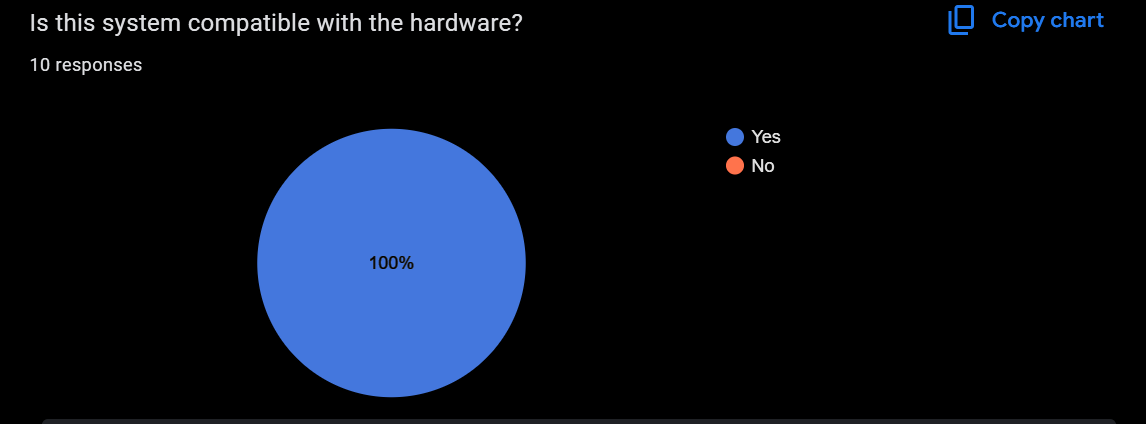
\includegraphics[width=0.7\textwidth]{Hardware.png}
    \caption{Participant Feedback for Hardware use}
    \label{FigUH}
\end{figure}

\begin{figure}[h]
    \centering
    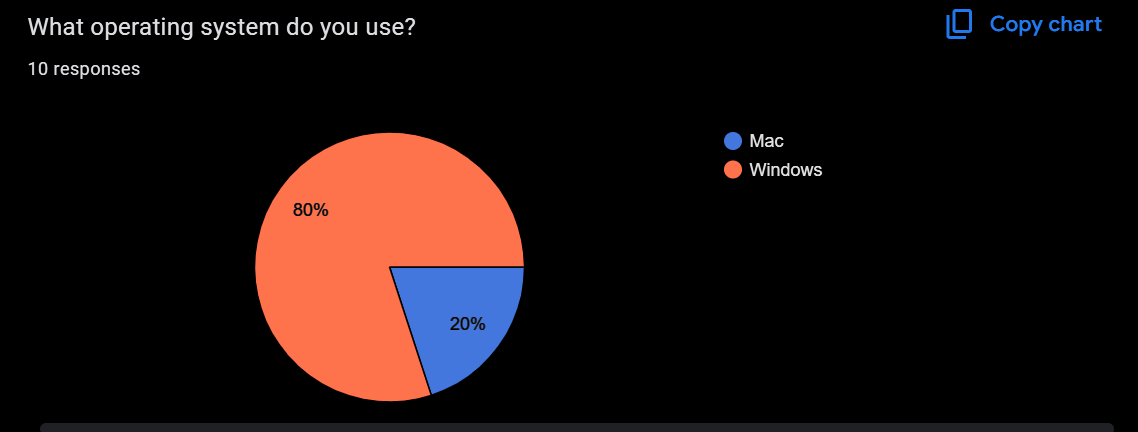
\includegraphics[width=0.7\textwidth]{Software.png}
    \caption{Participant Feedback for Software compatibility}
    \label{FigUH}
\end{figure}

\begin{figure}[h]
    \centering
    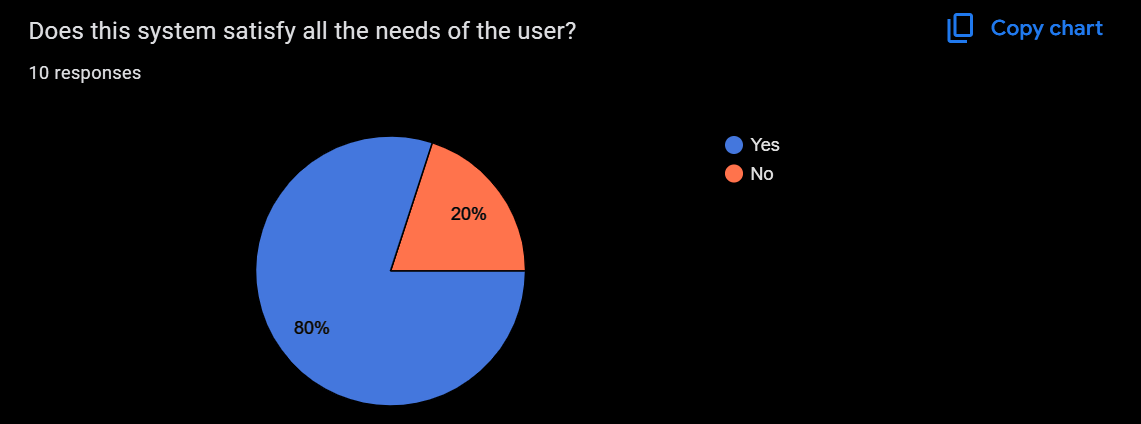
\includegraphics[width=0.7\textwidth]{UserNeeds.png}
    \caption{Participant Feedback for User Needs Satisfaction}
    \label{FigUH}
\end{figure}

\begin{figure}[h]
    \centering
    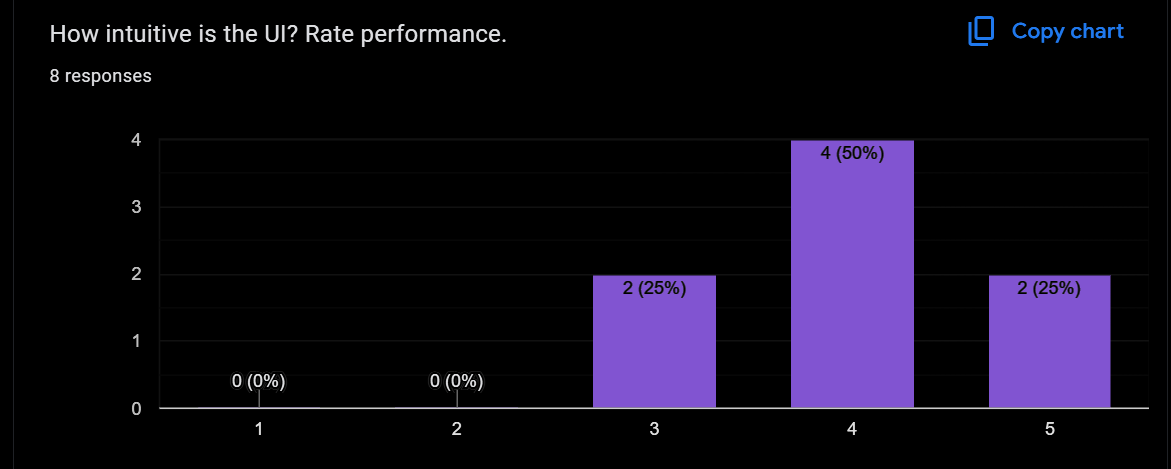
\includegraphics[width=0.7\textwidth]{UI.png}
    \caption{Participant Feedback for UI}
    \label{FigUH}
\end{figure}

\begin{figure}[h]
    \centering
    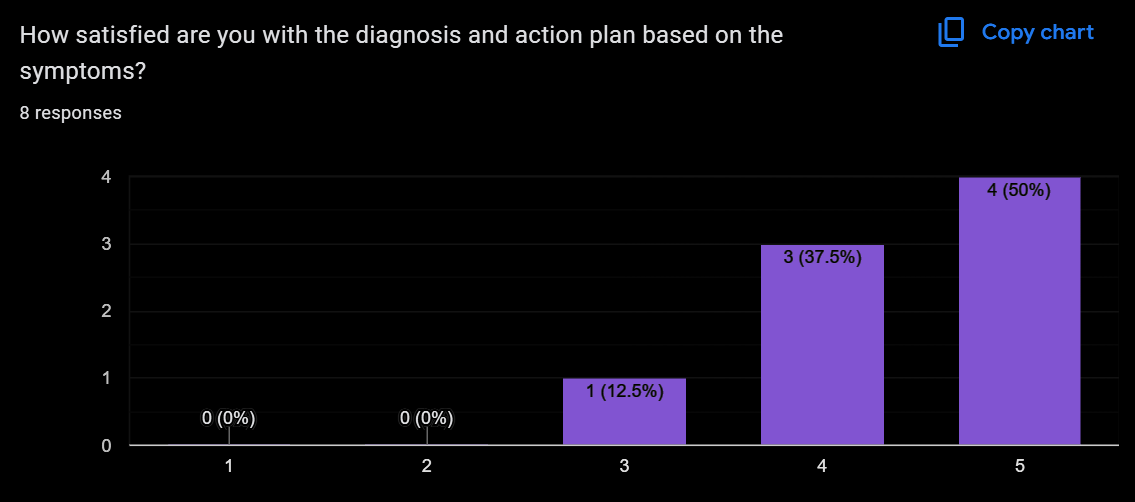
\includegraphics[width=0.7\textwidth]{DiagnosisAction.png}
    \caption{Participant Feedback for Diagnosis and Action plan prediction}
    \label{FigUH}
\end{figure}

\begin{figure}[h]
    \centering
    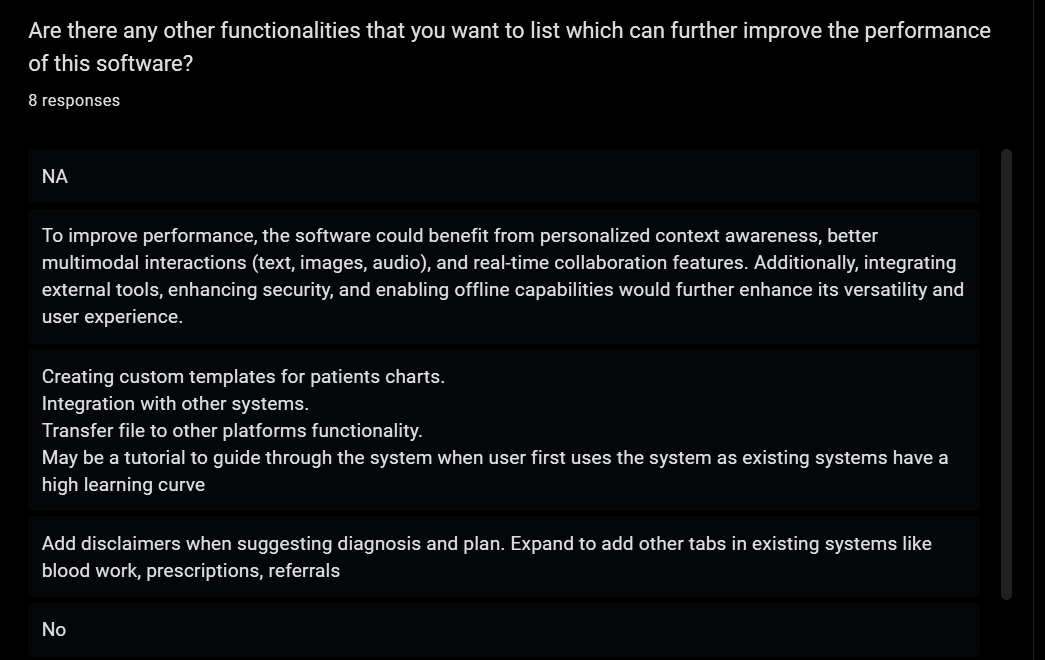
\includegraphics[width=0.7\textwidth]{Improvements.png}
    \caption{Participant Feedback for future improvements}
    \label{FigUH}
\end{figure}

\subsection{Issues}

There were no technical issues experienced with the software by any of the participants.

\newpage

\section{Recommendations}

The participants recommended different actions to further improve the software. The recommendations are listed below:

\begin{enumerate}
    \item To improve performance, the software could benefit from personalized context awareness, better multimodal interactions (text, images, audio), and real-time collaboration features. Additionally, integrating external tools, enhancing security, and enabling offline capabilities would further enhance its versatility and user experience.
    \item Creating custom templates for patients charts, integration with other systems, transferring files to other platforms functionalities could further improve the performance.
    \item May be a tutorial to guide through the system when user first uses the system as existing systems have a high learning curve.
    \item Add disclaimers when suggesting diagnosis and plan. Expand to add other tabs in existing systems like blood work, prescriptions, referrals.
    \item Multi-language support to support diverse cultural groups.
    \item The AI handle could be further modified for specific cases.
\end{enumerate}

\newpage

\section{Conclusion}

\subsection{Changes Implemented}

As a part of already implemented changes, the following changes are already/will be implemented.

\begin{enumerate}
    \item Based on the preliminary testing that we did with our supervisor before Rev 0 demo, the feedback we got was to create an AI functionality to assist in fetching patient data for the healthcare professional without manually reviewing the patient record.
    \item We also implemented the referrals and prescriptions tabs based on our supervisor's feedback.
    \item Another change that we will implement as a part of next steps is adding disclaimers in UI when the diagnosis and treatment plans will be predicted by the system.
    \item We will also make a user manual to assist first-time users who will be using this system.
\end{enumerate}

All the other suggestions from the feedback are noted and will be worked upon as a part of next steps.

\newpage

\bibliographystyle {plainnat}
\bibliography{../../../refs/References}

\end{document}